\documentclass[notes]{beamer}
\usepackage[utf8]{inputenc}
\usepackage{hyperref}
\usepackage[backend=biber, style=authoryear, sorting=none]{biblatex}
\usepackage{fancyhdr}
\usepackage{colortbl}
\usepackage{setspace}   % line space
\usepackage{algorithm}
\usepackage{algpseudocode}
\usepackage{float}
\usepackage{media9}
\usepackage{tikz}
\usefonttheme{professionalfonts}

\algnewcommand{\Inputs}[1]{%
    \State \textbf{Inputs:}
    \Statex \hspace*{\algorithmicindent}\parbox[t]{.8\linewidth}{\raggedright #1}
}
\algnewcommand{\Initialize}[1]{%
    \State \textbf{Initialize:}
    \Statex \hspace*{\algorithmicindent}\parbox[t]{.8\linewidth}{\raggedright #1}
}
\algnewcommand{\Outputs}[1]{%
    \State \textbf{Outputs:}
    \Statex \hspace*{\algorithmicindent}\parbox[t]{.8\linewidth}{\raggedright #1}
}

\setstretch{1.0}

\usetheme{Madrid}
\usecolortheme{default}


\graphicspath{{figures/}}	% set graph path

\addbibresource{references.bib}   % Inserting the references file
\renewcommand{\bibfont}{\normalfont\footnotesize}

% ------------------------------------------------------------
% headline
\setbeamertemplate{headline}
{
\begin{beamercolorbox}[wd=\paperwidth,ht=3.0ex,dp=1.325ex]{section in head/foot}%
\usebeamerfont{subsection in head/foot}\insertsectionnavigationhorizontal{\paperwidth}{}{}
\end{beamercolorbox}
}

%------------------------------------------------------------
% color
\definecolor{purple}{RGB}{206, 87, 193}
\definecolor{black}{RGB}{0, 0, 0}
\definecolor{white}{RGB}{255, 255, 255}
\definecolor{red}{RGB}{215, 0, 0}
\definecolor{yellow}{RGB}{255, 242, 0}


%------------------------------------------------------------
%This block of code defines the information to appear in the
%Title page
\title %optional
{Information Bottleneck}

\subtitle{}

\author[Yangshuo He] % (optional)
{Yangshuo He}

\institute[UoM] % (optional)
{
    The University of Melbourne
    \and
    Department of Electrical and Electronic Engineering
}

\usepackage{datetime}
\renewcommand{\today}{\twodigit{\day}/\twodigit{\month}/\number\year}
\date{\today}

% \logo{\includegraphics[height=1cm]{overleaf-logo}}

%End of title page configuration block
%------------------------------------------------------------



%------------------------------------------------------------
%The next block of commands puts the table of contents at the 
%beginning of each section and highlights the current section:

% \AtBeginSection[]
% {
%   \begin{frame}
%     \frametitle{Table of Contents}
%     \tableofcontents[currentsection]
%   \end{frame}
% }
%------------------------------------------------------------


\begin{document}



%The next statement creates the title page.
\frame{\titlepage}

\section{Introduction}

%---------------------------------------------------------
%This block of code is for the table of contents after
%the title page
\begin{frame}
\frametitle{Outline}
\begin{itemize}
    \item Background of the Information Bottleneck (IB) framework
    \item The IB cracks open the black box of deep learning
    \begin{itemize}
        \item Two phases of the information dynamics during training
        \item An information compression bounds
    \end{itemize}
    \item Ongoing debates on the IB framework
\end{itemize}
\begin{figure}
    \centering
    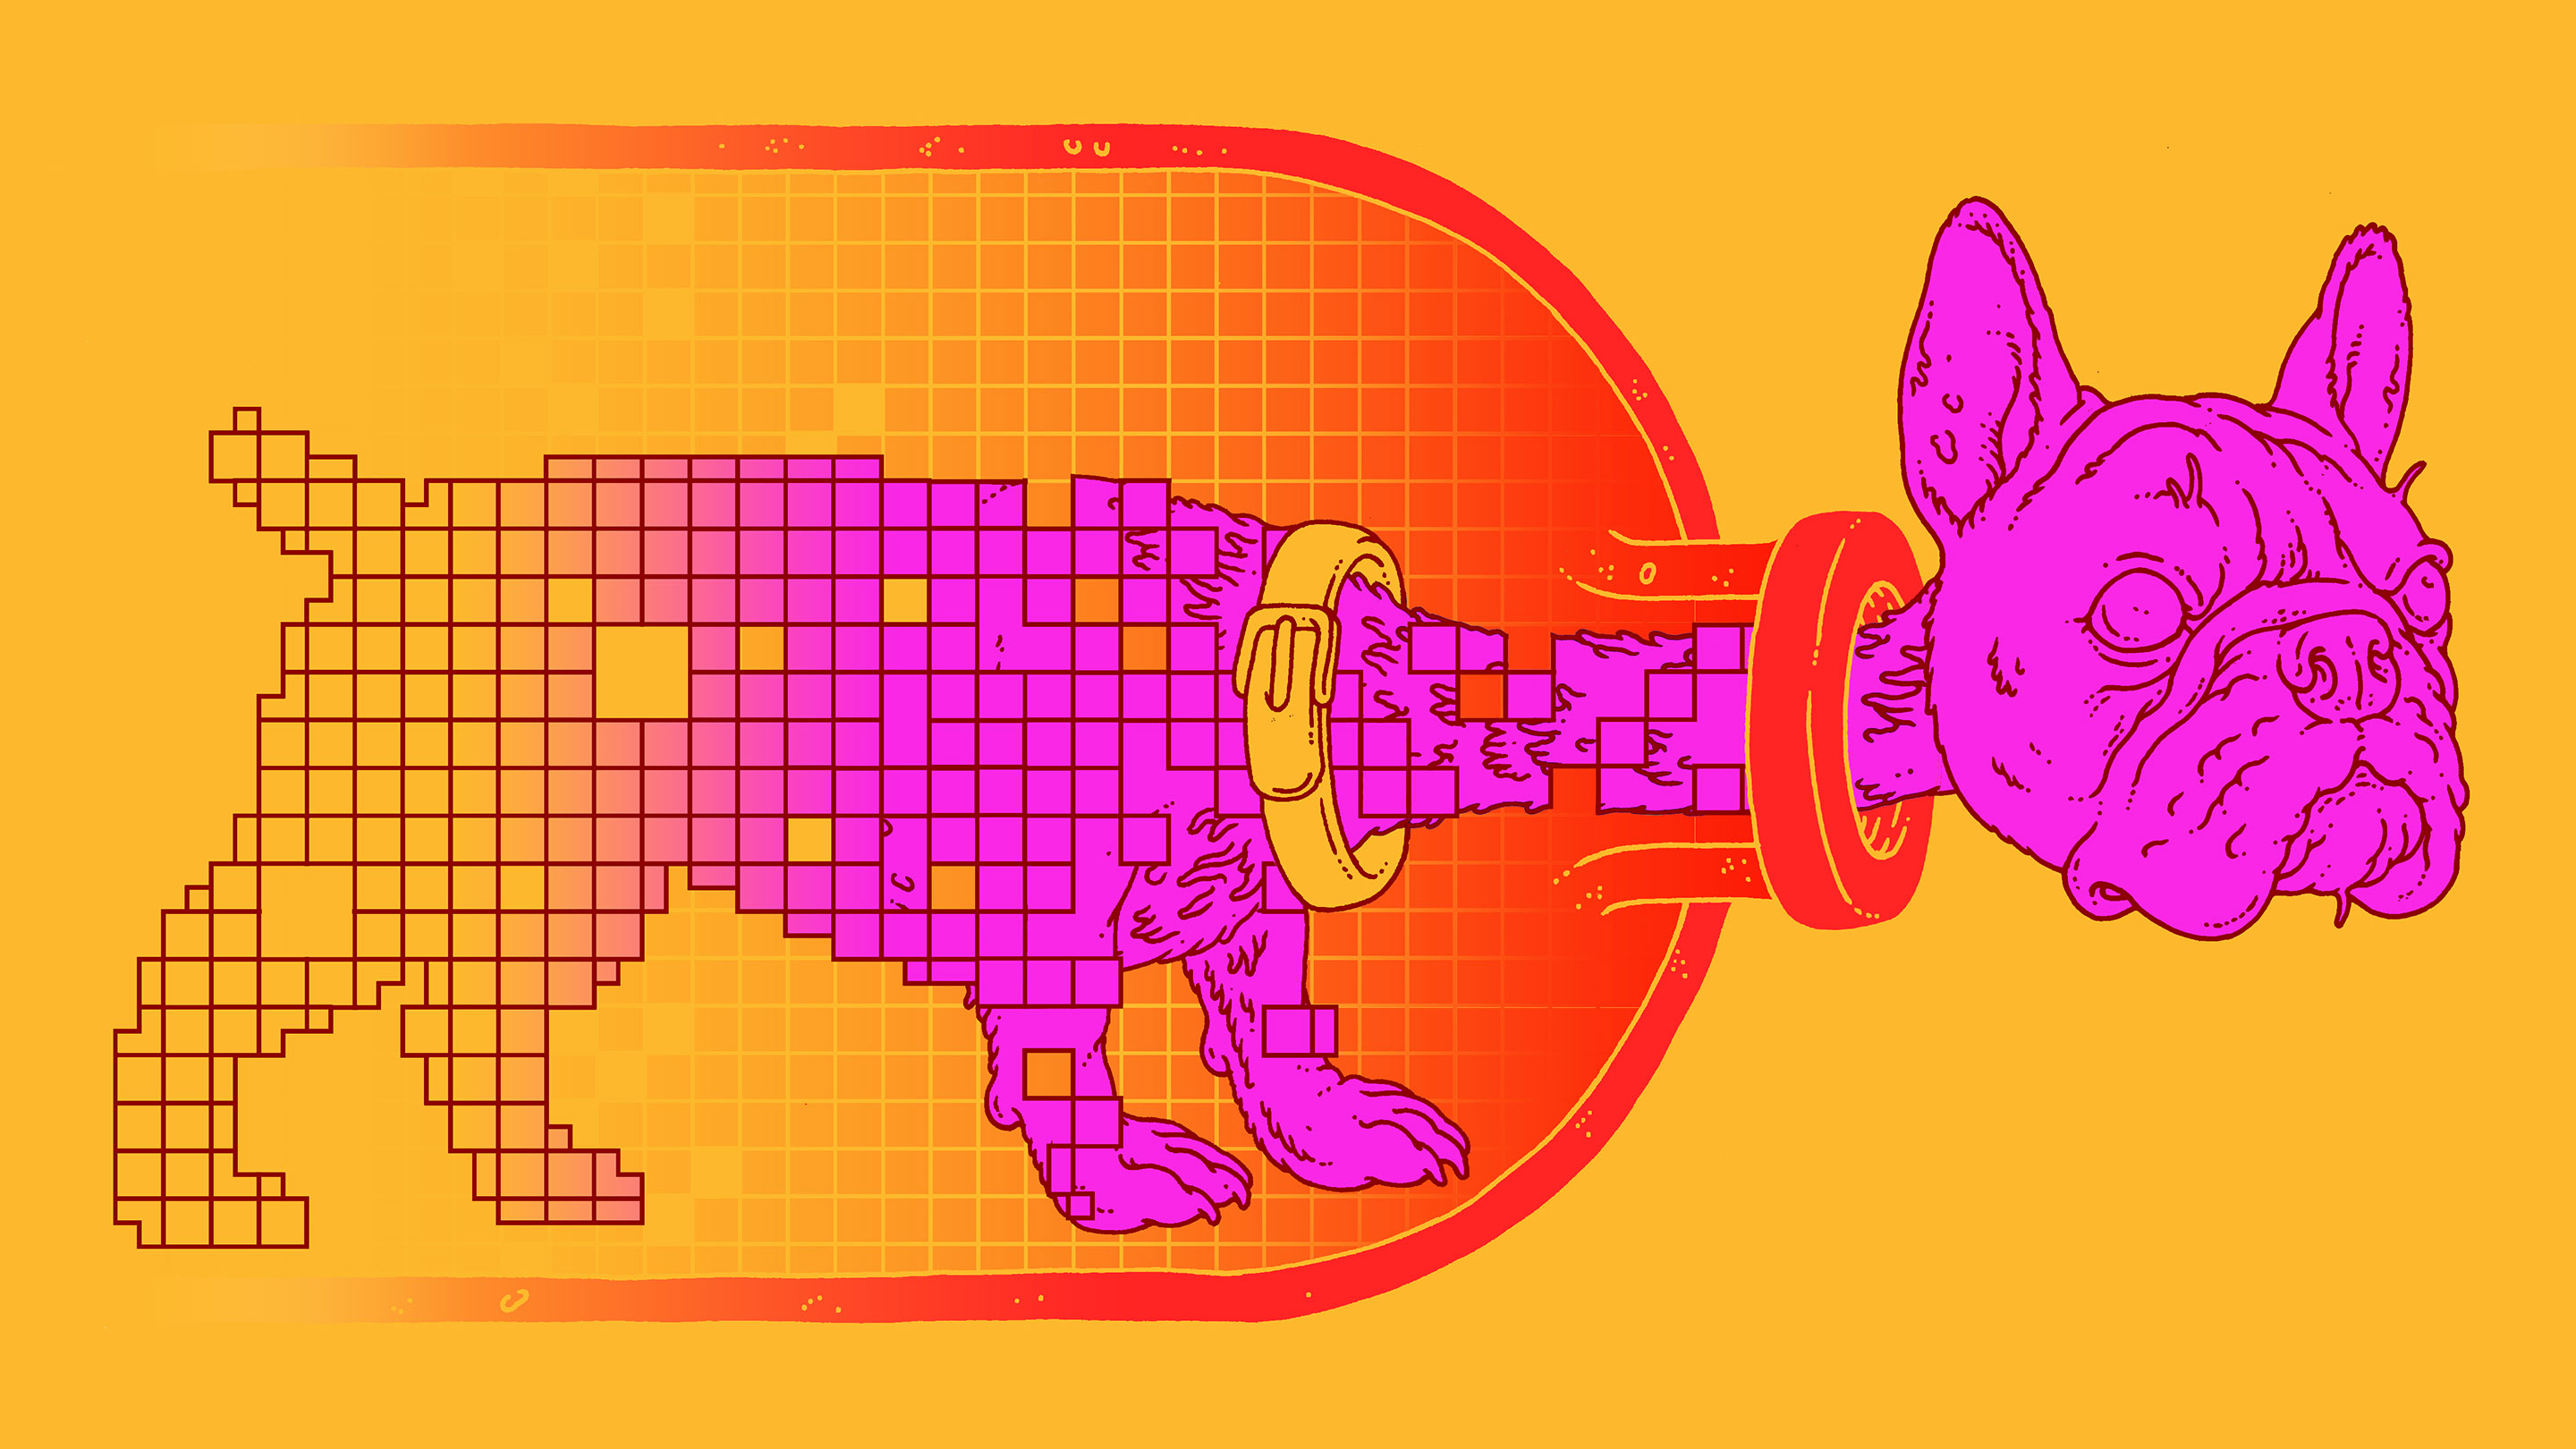
\includegraphics[width=6cm]{IB_dog.jpg}
\end{figure}
\end{frame}

%---------------------------------------------------------



%---------------------------------------------------------

\begin{frame}
    \frametitle{How does DNN work?}
    \begin{itemize}
        \item Deep learning (DL) has shown its great potential in learning critical information for certain tasks \note{The magic of DNN is its generalization ability: learning from special cases, while showing intelligence toward general concepts.}
        \item The theoretical understanding of DL remains unsatisfied \note{DNN is a black box.}
        \item Information theory plays an important role in explaining the DL mechanism \note{DL is actually extracting patterns from a large scale complex data, it involves data commpression, has similar concept of encoding and decoding}
    \end{itemize}
\end{frame}

%---------------------------------------------------------

\begin{frame}
    \frametitle{IB combines 3 different ingredients}
    \begin{itemize}
        \item Learning Theory: data-dependent but architecture-independent bound \note{from worst case results to a typical case result}
        \item Information Theory: using the same notations and techniques
        \item Stochastic dynamics of the training: convergence of SGD
    \end{itemize}
\end{frame}


\section{Preliminaries}
%---------------------------------------------------------

\begin{frame}
\frametitle{Review of DNN}
\begin{columns}
    \begin{column}{0.65\textwidth}
        \begin{figure}
            \centering
            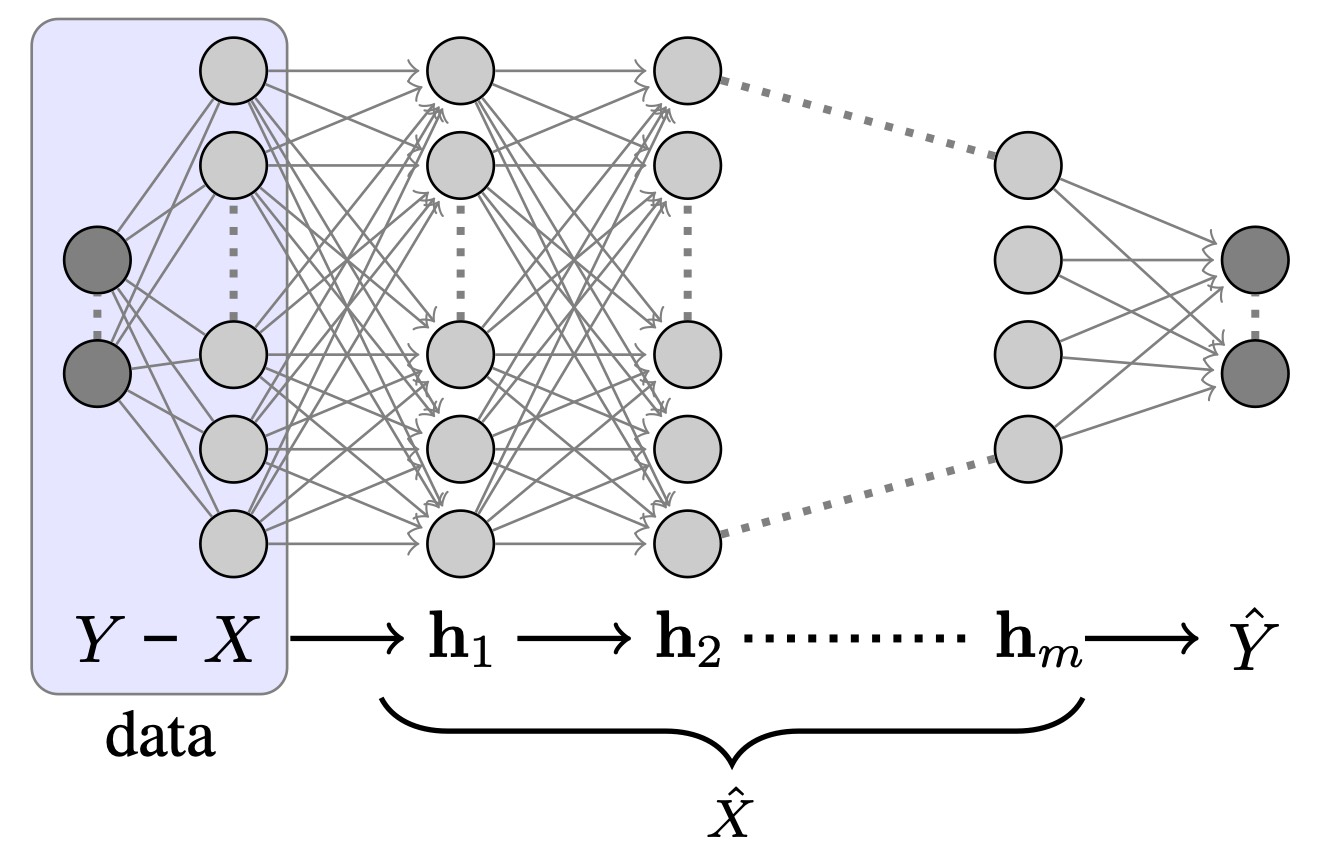
\includegraphics[width=6cm]{DNN.jpg}
        \end{figure}
    \end{column}
    \begin{column}{0.35\textwidth}
        \begin{itemize}
            \item $Y$: target label
            \item $X$: input data
            \item $\mathbf{h}_i$: features
            \item $\hat{Y}$: prediction
        \end{itemize}
    \end{column}
\end{columns}
\begin{itemize}
    \item The input data goes through a series of transformations
    \begin{equation}
        \mathbf{h}_{i+1}=\sigma(W_i\mathbf{h}_{i}+b_i),\quad \mathbf{h}_0=X
    \end{equation}
    \note{Each layer generates a new representation of the input data}
    \item The cascade network forms a \textbf{Markov chain}
    \begin{equation}
        Y\to X\to \hat{X}\to \hat{Y}
    \end{equation}
    \note{The prediction Markov chain is incorrect, $X\to\hat{X}\to Y$}
\end{itemize}
\note{$X$ is a high entropy random variable, $Y$ is a simple low dimensional variable. The last layer generate a random variable, as close as $Y$.}
\note{Each representation is calculated by the previous one, and only affect the next one.}
\note{If the training works well, this series of refinement of data, lead to a good prediction.}
\note{The IB framework focuses on what really happens for these intermediate representations.}
\end{frame}


%---------------------------------------------------------


%---------------------------------------------------------

\begin{frame}
    \frametitle{Information Theory Basics}
    
    \begin{itemize}
        \item The KL divergence: for any two distributions $p$ and $q$ over $\mathcal{X}$:
        \begin{equation*}
            D\left(p \| q\right) = \sum_{x\in\mathcal{X}} p(x) \log \frac{p(x)}{q(x)} \ge 0
        \end{equation*}
        \item The mutual information: for any two r.v.s $X$ and $Y$:
        \begin{equation*}
            I(X;Y)=D\left(p(x,y) \| p(x)p(y)\right) = H(X) - H(X|Y)
        \end{equation*}
        \item Data Processing Inequality (DPI): for any Markov chain $X\to Y\to Z$
        \begin{equation*}
            I(X;Y)\geq I(X;Z)
        \end{equation*}
    \end{itemize}
    
\end{frame}

%---------------------------------------------------------

\begin{frame}
    \frametitle{The IB Method (\cite{IB-method})}
    \note{The IB method was introduced long ago, which originated from the Rate-Distortion problem. The key difference is the introduction of an additional variable that dtermines what is relevant.}
    \begin{columns}[T]
        \begin{column}{0.5\textwidth}
            \begin{itemize}
                \item Standard compression
                \begin{equation*}
                    X\to \hat{X}
                \end{equation*}
                \item A constraint through a distance function:
                \begin{equation*}
                    \mathcal{L}\left[p\left(\hat{x}|x\right)\right] \!=\! I(X;\hat{X}) + \beta \mathbb{E}\left[d\left(x,\hat{x}\right)\right]
                \end{equation*}
            \end{itemize}
        \end{column}
        \begin{column}{0.5\textwidth}
            \begin{itemize}
                \item Relevance compression
                \begin{equation*}
                    Y\to X\to \hat{X}
                \end{equation*}
                \item A constraint on the meaningful information:
                \begin{equation*}
                    \mathcal{L}\left[p\left(\hat{x}|x\right)\right] \!=\! I(X;\hat{X}) - \beta I(\hat{X};Y)
                \end{equation*}
            \end{itemize}
        \end{column}
    \end{columns}
    \hspace{1cm}
    \begin{itemize}
        \item Using the Lagrange multipliers method, the optimal solution is
        \begin{equation}
            p^*(\hat{x}|x) = \frac{p(\hat{x})}{Z(x, \beta)} \exp\left[-\beta D\left(p(y|x)\|p(y|\hat{x})\right)\right],
        \end{equation}
        where $Z(x, \beta)$ is the normalization function
        \item Iteratively solved by Blauht-Arimoto algorithm
    \end{itemize}
    \note{These two methods are equivalent when we choose a KL divergence distortion $d_{IB}\left(x,\hat{x}\right)=D\left(p(y|x)\|p(y|\hat{x})\right)$.}
\end{frame}

\section{Main Results}

\begin{frame}
    \frametitle{What do the DNN layers represent?}
    \begin{columns}
        \begin{column}{0.4\textwidth}
            \begin{figure}
                \centering
                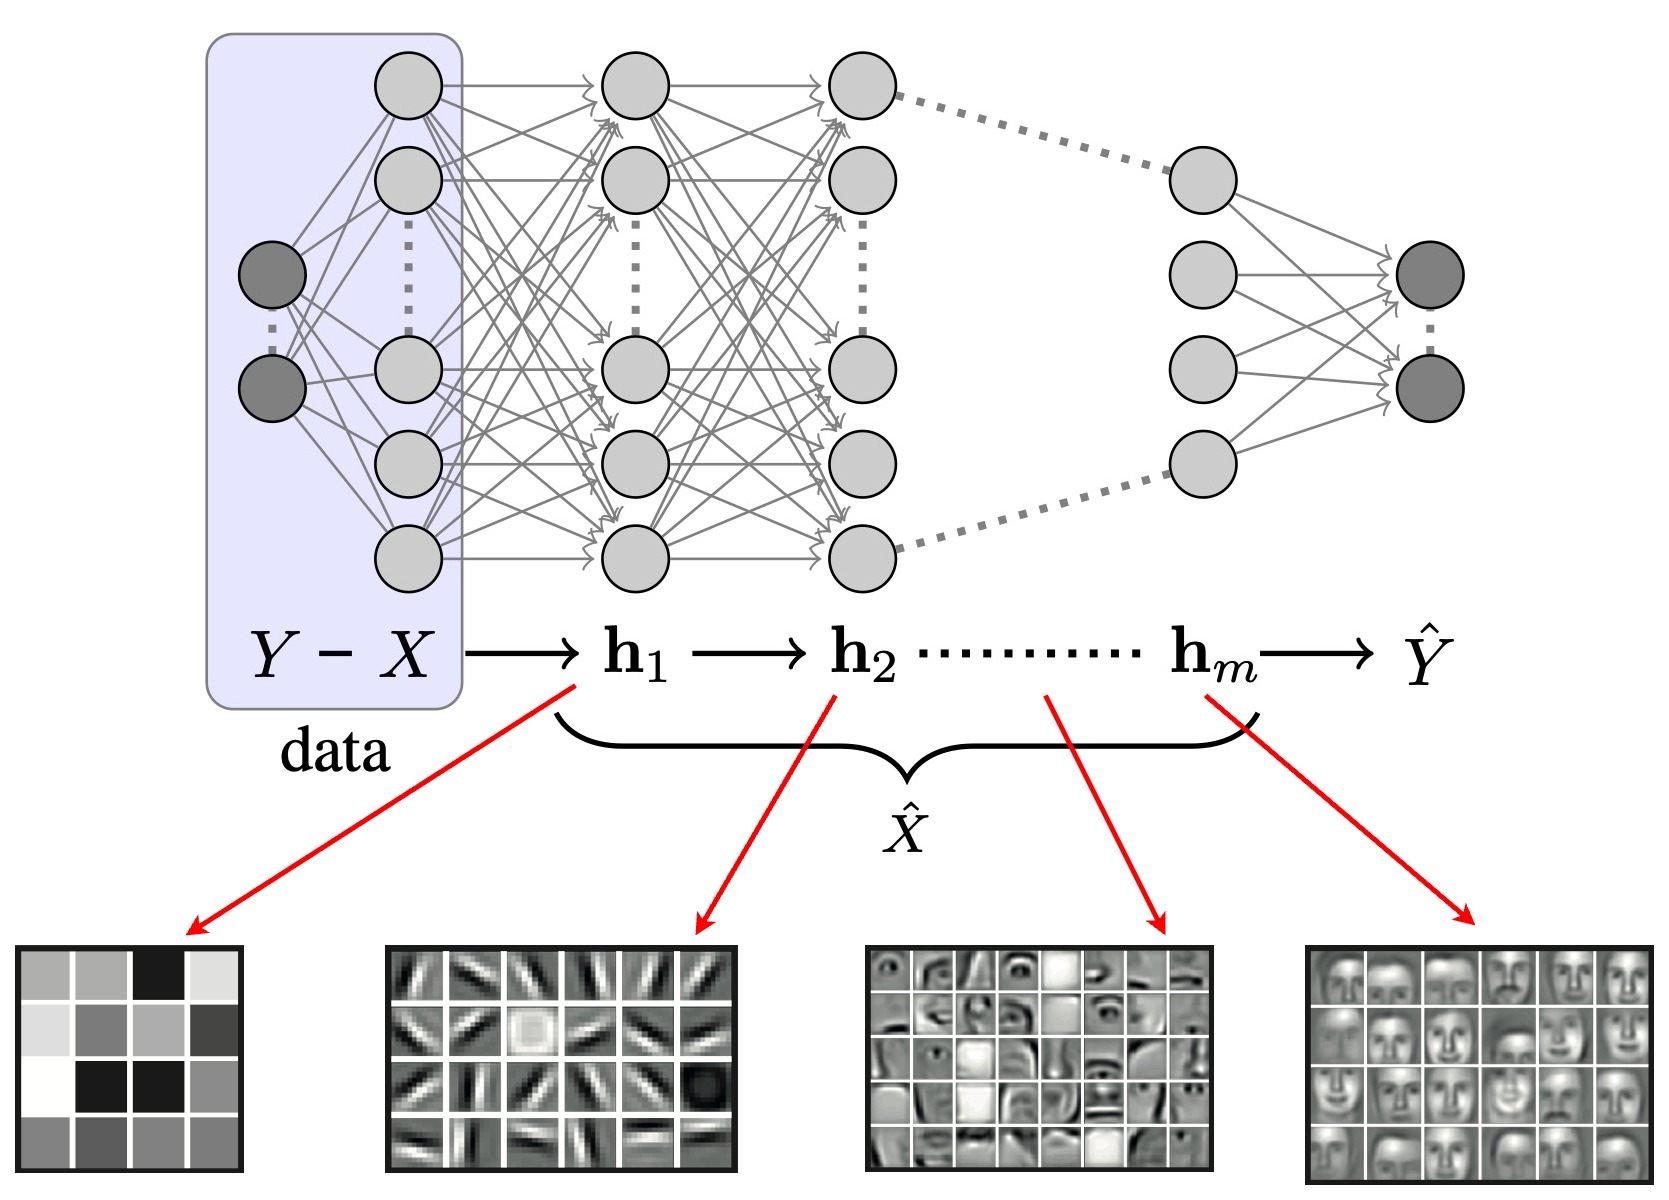
\includegraphics[width=5.5cm]{DNN_partition.jpg}
            \end{figure}
        \end{column}
        \begin{column}{0.6\textwidth}
            \begin{itemize}
                \item Apply DPI on the cascade representations:
                \begin{align}
                    & H(X)\geq I(X;\mathbf{h}_{i}) \geq I(X;\mathbf{h}_{i+1})\geq\cdots \\
                    & I(X;Y) \geq I(\mathbf{h}_{i};Y) \geq I(\mathbf{h}_{i+1};Y)\geq \cdots 
                \end{align}
                \item Each layer gives a more refine representation
                \item These representations induce distinct partitions of input
            \end{itemize}
        \end{column}
    \end{columns}
    \note{Now, let's go back to the DNN, and take a look at what do the layers represent and how IB method related to DNN?}
    \note{When we look back to these cascade representation, we would find out two chains of inequalities. We will calculate the mutual information of each layer between the input data $X$ and target label $Y$.}
    \note{The equality in (5) is achievable if each layer representation is a sufficient minimal statistics.}
\end{frame}

\begin{frame}
    \frametitle{Consider a DNN as a pair of encoder and decoder}
    \begin{figure}
        \centering
        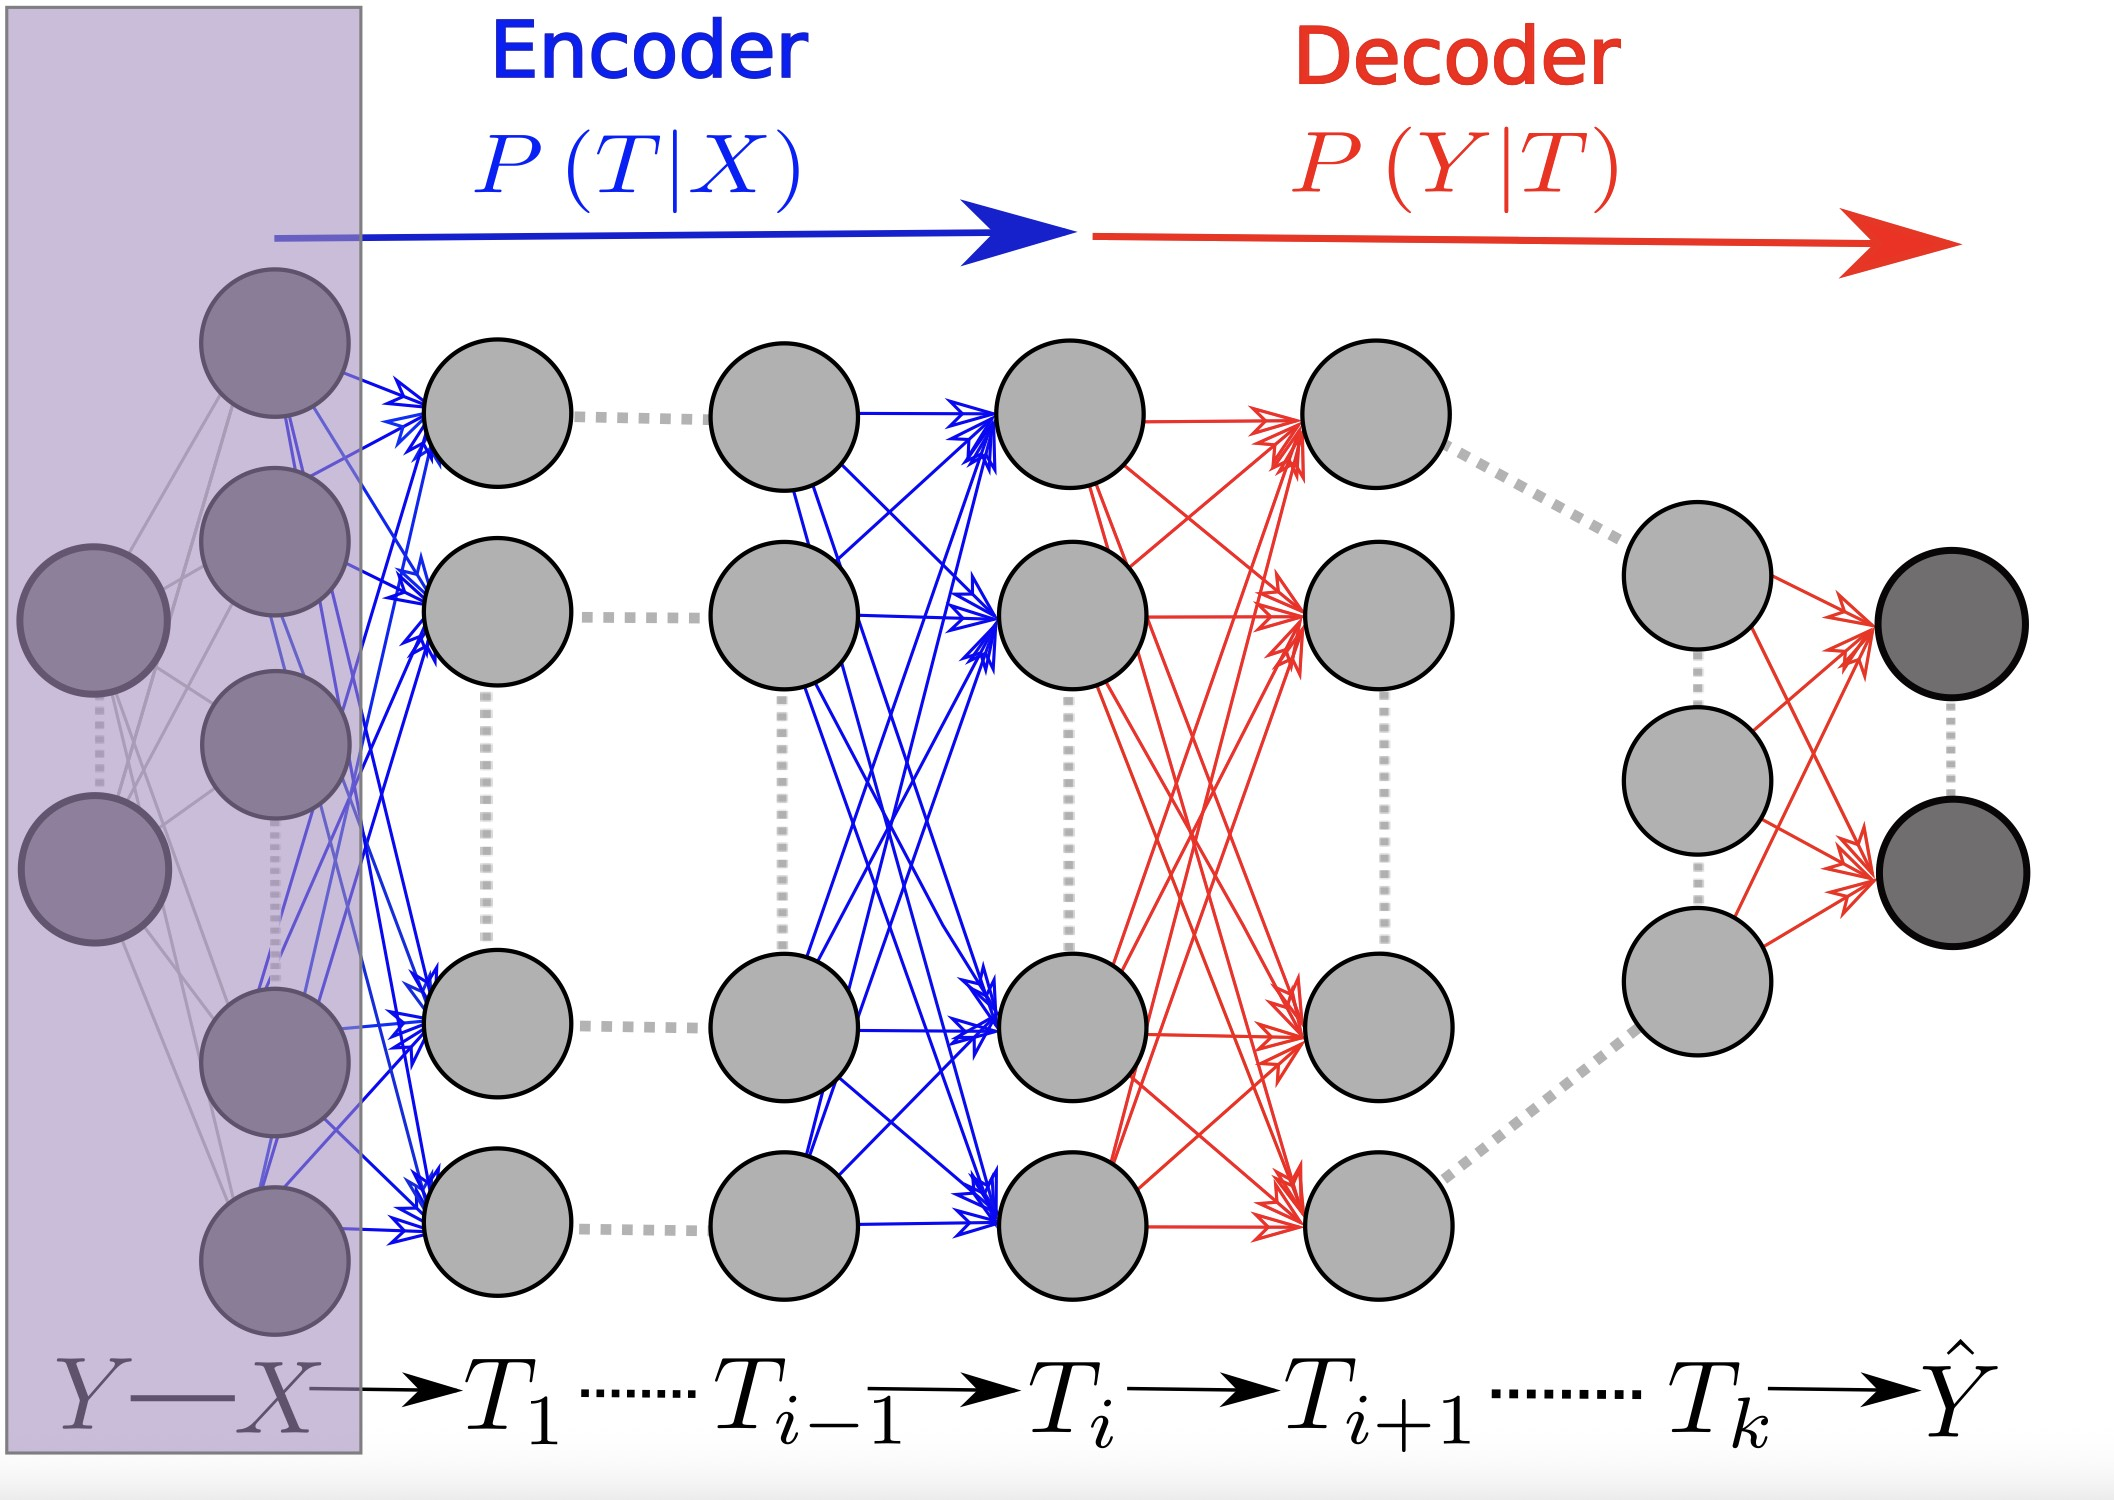
\includegraphics[width=5.5cm]{IB_encoder_decoder.jpg}
    \end{figure}
    \vspace{-0.2cm}
    \begin{itemize}
        \item A resemblance between DNN and relevance compression
        \item Learn a minimal sufficient statistics $T$ (\textbf{bottleneck}): minimal description length $I(X;T)$ and maximal relevant information $I(T;Y)$
    \end{itemize}
    \vspace{-0.2cm}
    \begin{block}{Statement (\cite{IB-DNN})}
        The sample complexity of DNN is determined by the encoder MI $I(X;T)$, and the accuracy is determined by the decoder MI $I(T;Y)$
    \end{block}
\end{frame}

\begin{frame}
    \frametitle{The Information Planes}
    \begin{itemize}
        \item IB framework formulates a trade-off between $I(X;T)$ and $I(T;Y)$
        \item The set of all possible pairs of MIs for any encoder $p(T|X)$ is called the \textbf{information plane}
    \end{itemize}
    \centering
    \includemedia[
        activate=pageopen,      % Start playing when the slide is opened
        addresource=IB_information_plane.mp4,
        flashvars={
            source=IB_information_plane.mp4
            &autoPlay=false
            &loop=false
            &controlBarMode=floating % Or 'docked', 'none'
            &playButton=true    % Show a prominent play button
            &initialframe=1     % Revert to the first frame (poster) after playing
        }
    ]{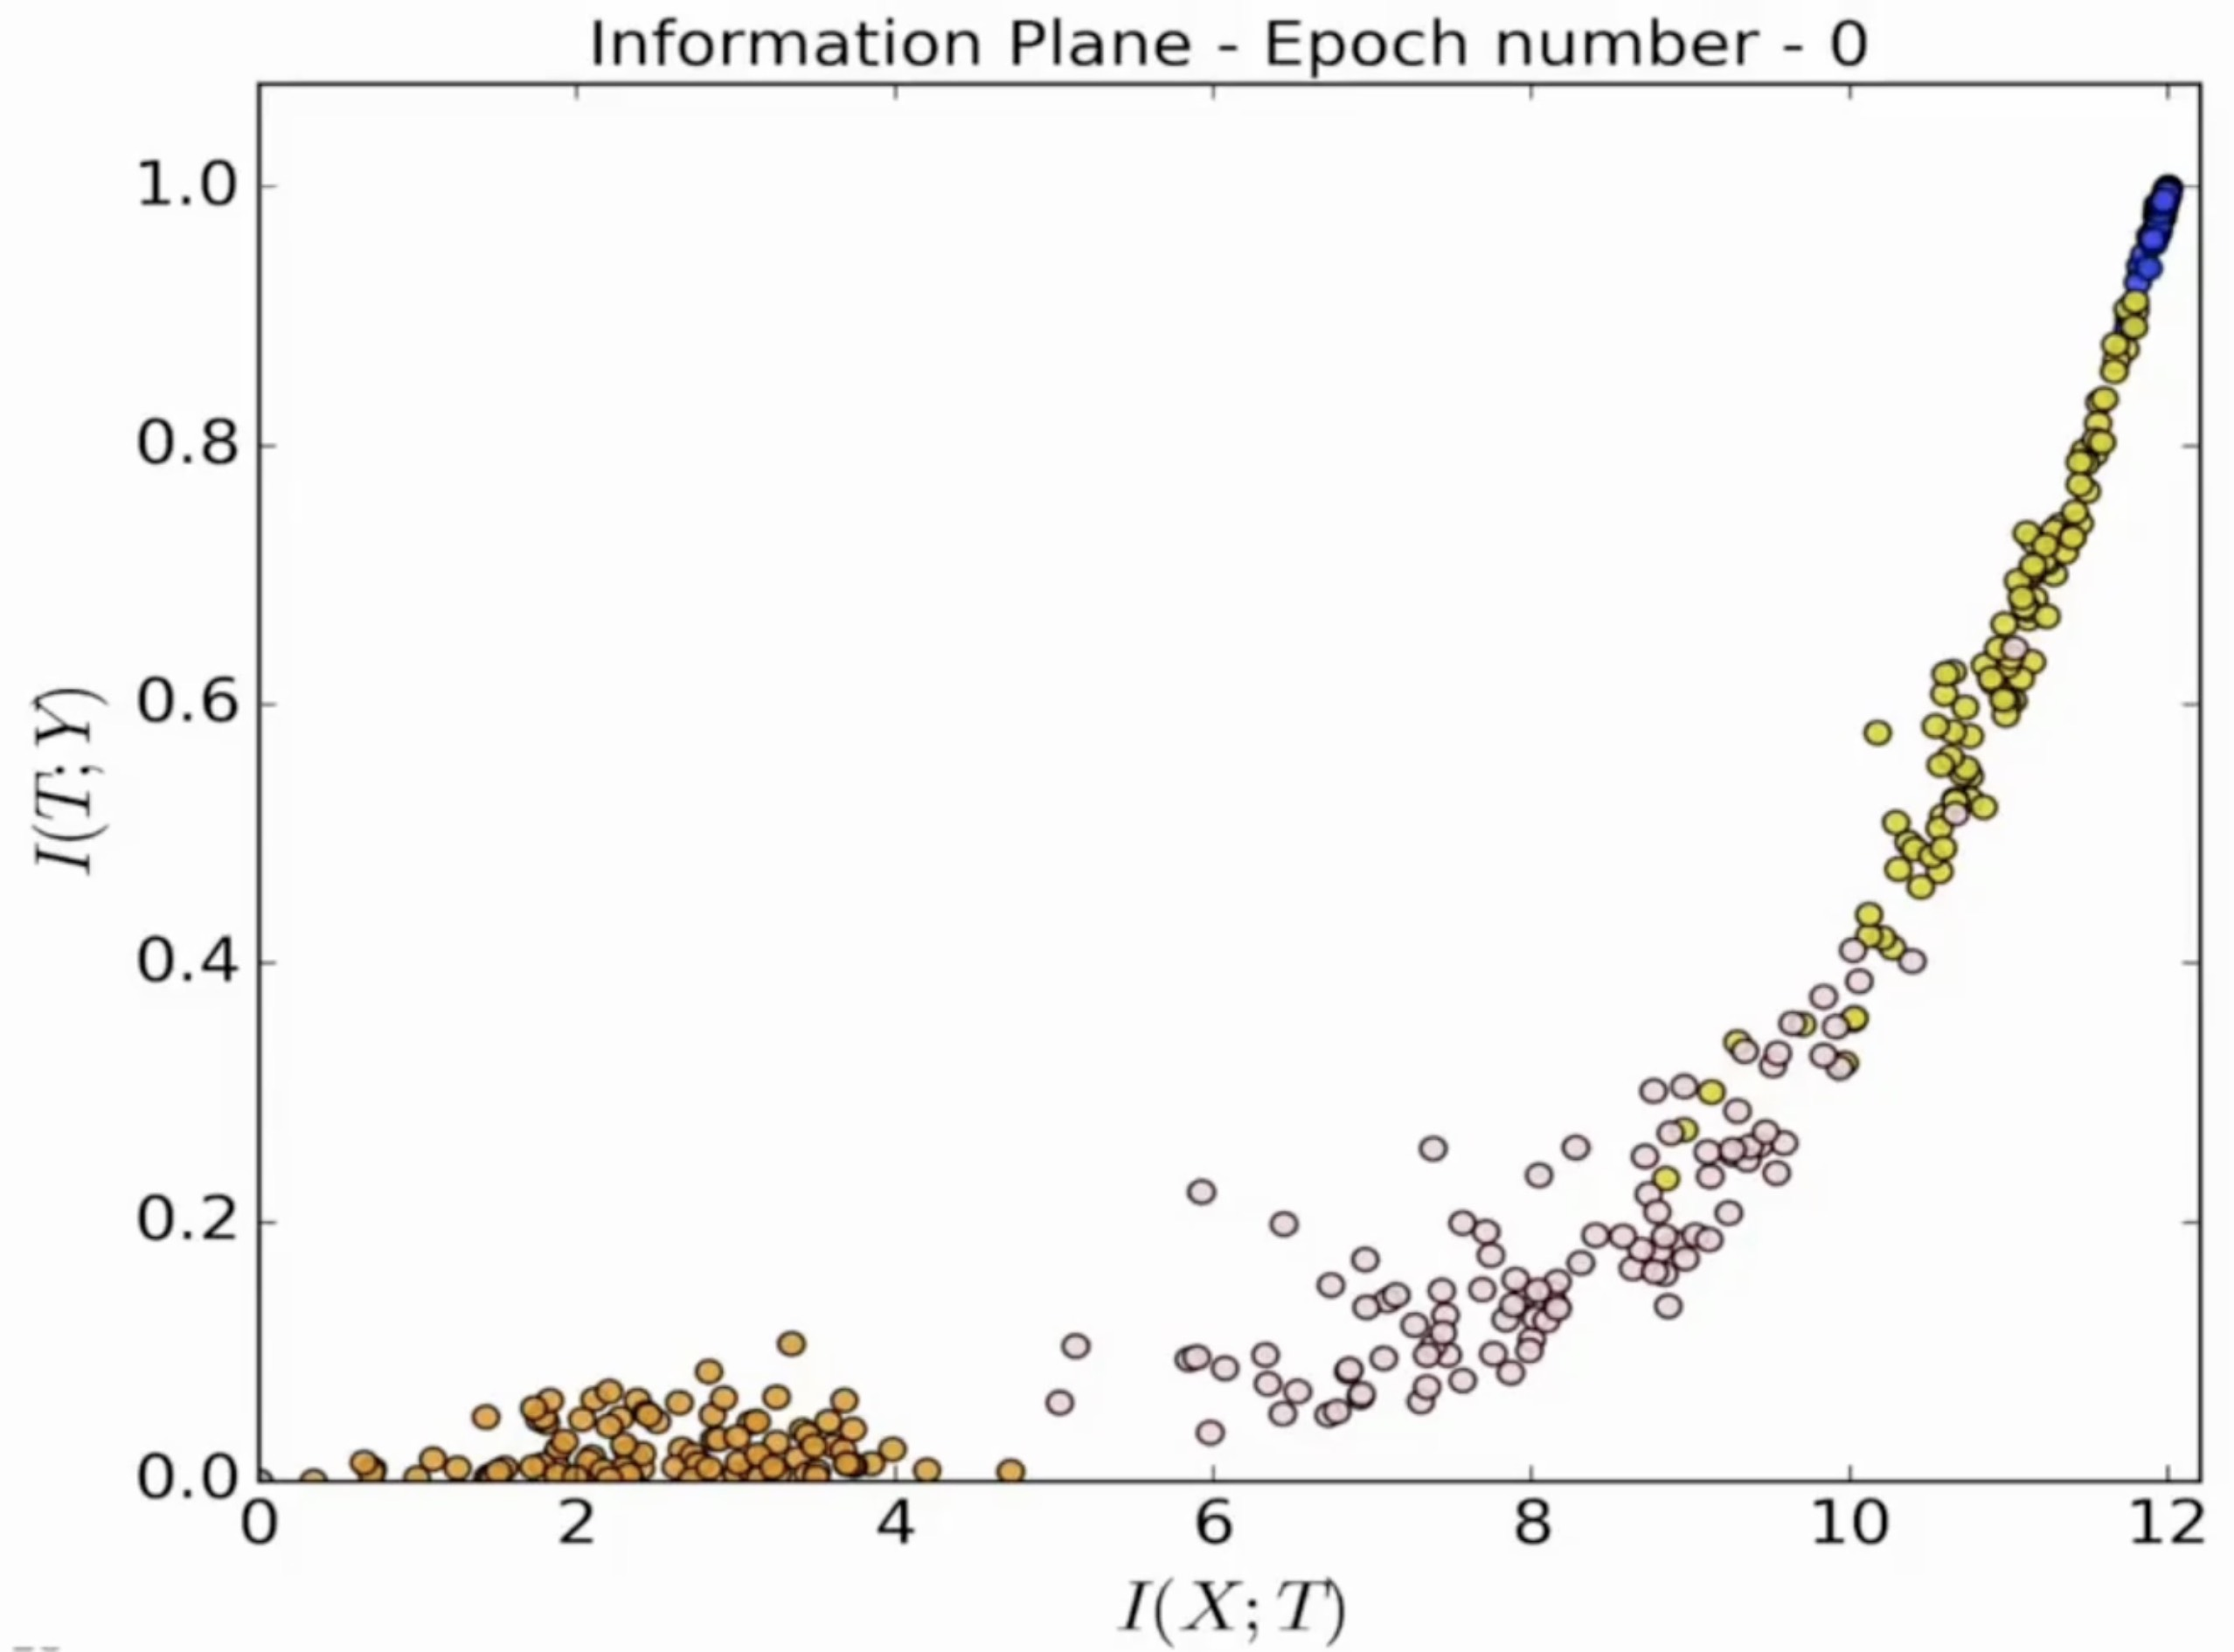
\includegraphics[width=0.6\textwidth]{IB_information_plane_poster.jpg}}{VPlayer.swf}
    \note{Each point represents a different initial condition. The points in the same color come from the same layer. The first layer is on the very right side, and the last layer is on the left. A simple binary decision task, input are 12 binary bits. A 7-layer DNN, with 12-10-7-5-4-3-2 neutrons each layer. The rule makes sure that the mutual information is close to 1 ($p(x)$ is uniform, and $p(y=1)\approx 0.5$). The training uses the traditional SGD algorithm without any regularization or dropout.}
    \begin{itemize}
        \item Simulations demonstrate a two phases dynamics during training
    \end{itemize}
\end{frame}

\begin{frame}
    \frametitle{Information Dynamics}
    \begin{columns}
        \begin{column}{0.5\textwidth}
            \begin{figure}
                \centering
                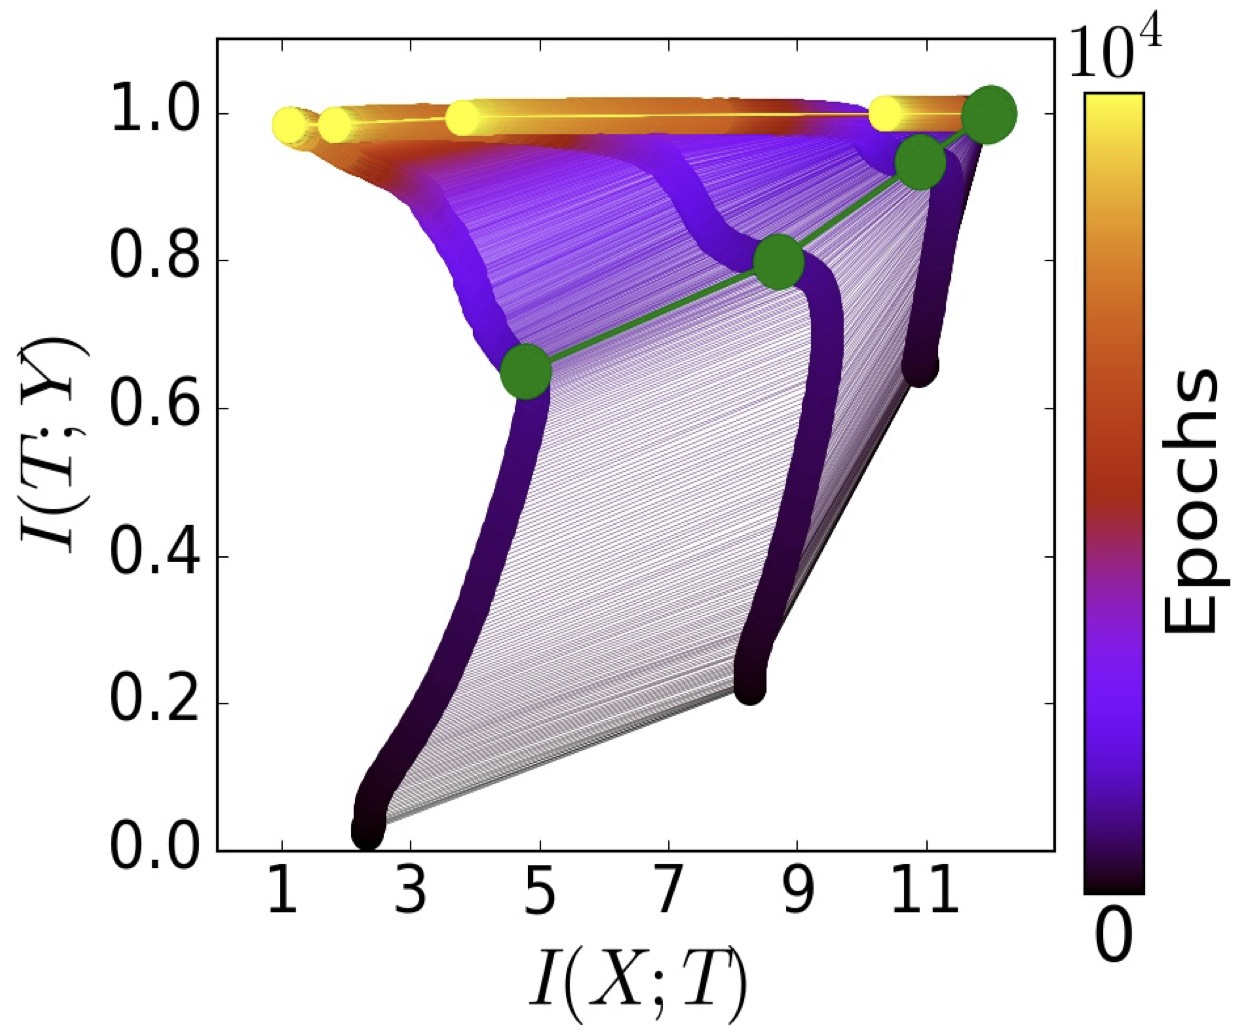
\includegraphics[width=6cm]{IB_information_plane.jpg}
            \end{figure}
        \end{column}
        \begin{column}{0.45\textwidth}
            \begin{itemize}
                \item \textbf{Fitting Phase:} the layers increase the information on the labels \note{a fast process, the representations learn information from both the labels and the data, while preserving the DPI order.}
                \item \textbf{Compression Phase:} the layers lose irrelevant information about data \note{a slow process until convergence}
            \end{itemize}
            \note{The first phase is reasonable since the ERM algorithm, but for the second phase requires an explanation.}
        \end{column}
    \end{columns}

\end{frame}

\begin{frame}
    \frametitle{Rethinking Learning Theory (Intuitively)}
    \begin{columns}[T]
        \begin{column}{0.45\textwidth}
            \begin{itemize}
                \item ``Old'' Generalization bound:
                \begin{equation*}
                    \epsilon^2 \leq \frac{\log|H|+\log\frac{2}{\delta}}{2m}
                \end{equation*}
                \item $\epsilon$: generalization error
                \item $|H|$: size of hypothesis space
                \item $m$: number of training samples
                \item $\delta$: confidence
                \item \textbf{Don't work for DL!} \note{The high dimension makes the bound vacuous.}
            \end{itemize}
        \end{column}
        \begin{column}<2->{0.55\textwidth}
            \begin{itemize}
                \item Input Compression bound:
                \item $|H|\sim 2^{|X|}\to 2^{|T|}$
                \item Typical set and typical partition
                \begin{align*}
                    p(x_1,\cdots,x_n) & \approx 2^{-nH(X)}\\
                    p(x_1,\cdots,x_n|T)& \approx 2^{-nH(X|T)}
                \end{align*}
                \item The size of partition $|T|\sim 2^{I(X;T)}$
                \begin{equation*}
                    \epsilon^2\leq \frac{2^{I(X;T)}+\log\frac{2}{\delta}}{2m}
                \end{equation*}
                \item every bit of compression is like doubling the training samples.
            \end{itemize}
        \end{column}
    \end{columns}
    \begin{tikzpicture}[remember picture, overlay]
        % The <2-> makes this node appear only on slide 2
        \node<2-> at (current page.south west) [anchor=south west, xshift=0.2cm, yshift=0.5cm] {
            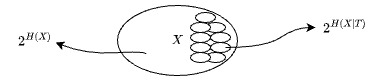
\includegraphics[width=6cm]{typical.jpg}
        };
    \end{tikzpicture}
\end{frame}

\begin{frame}
    \frametitle{Interesting Results}
    \vspace{-0.25cm}
    \begin{figure}
        \centering
        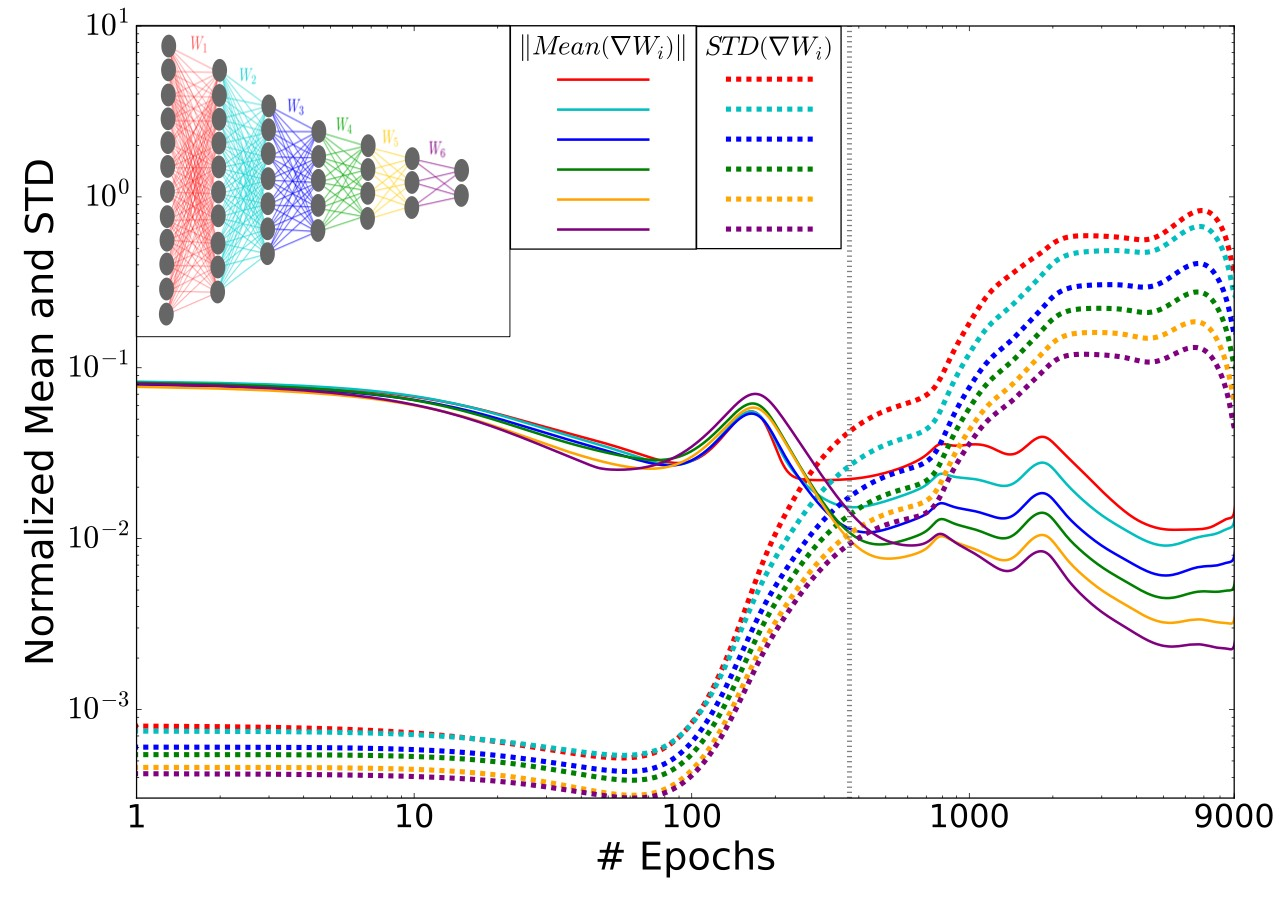
\includegraphics[width=8cm]{mean_std.jpg}
    \end{figure}
    \vspace{-0.4cm}
    Two clear phases during training: 
    \begin{itemize}
        \item High SNR phase: memorization (drift)
        \item Low SNR phase: forgetting (diffusion)
    \end{itemize}
    \textbf{Claim: These two stochastic gradient phases correspond the fitting and compression phases}
\end{frame}

\begin{frame}
    \frametitle{Interesting Results}
    \begin{figure}
        \centering
        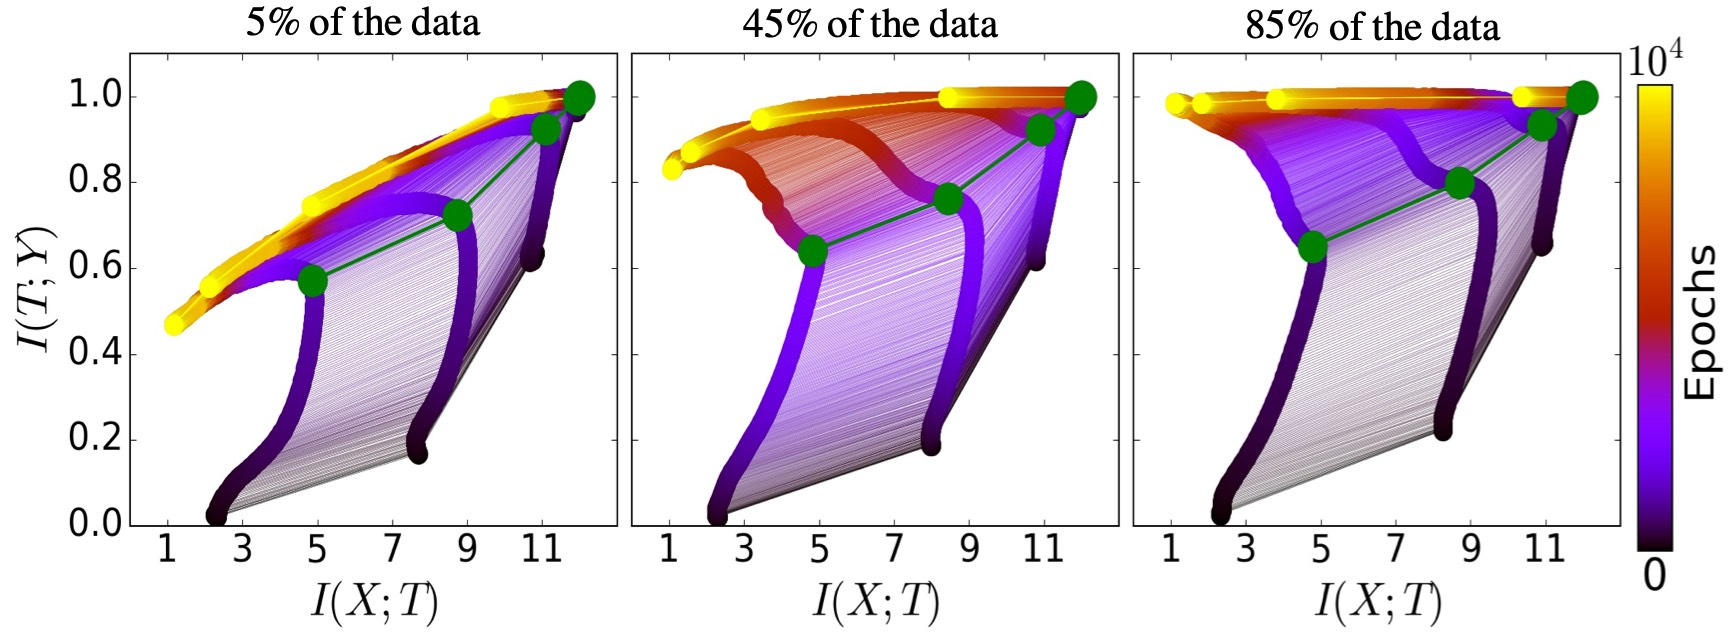
\includegraphics[width=10cm]{info_plane_data.jpg}
    \end{figure}
    The information dynamics of the layers, for different training samples
    \begin{itemize}
        \item The initial fitting phases are similar
        \item Lack of training data causes over-compression (over-fitting) in the compression phase
    \end{itemize}
\end{frame}

\begin{frame}
    \frametitle{Interesting Results}
    \vspace{-0.25cm}
    \begin{figure}
        \centering
        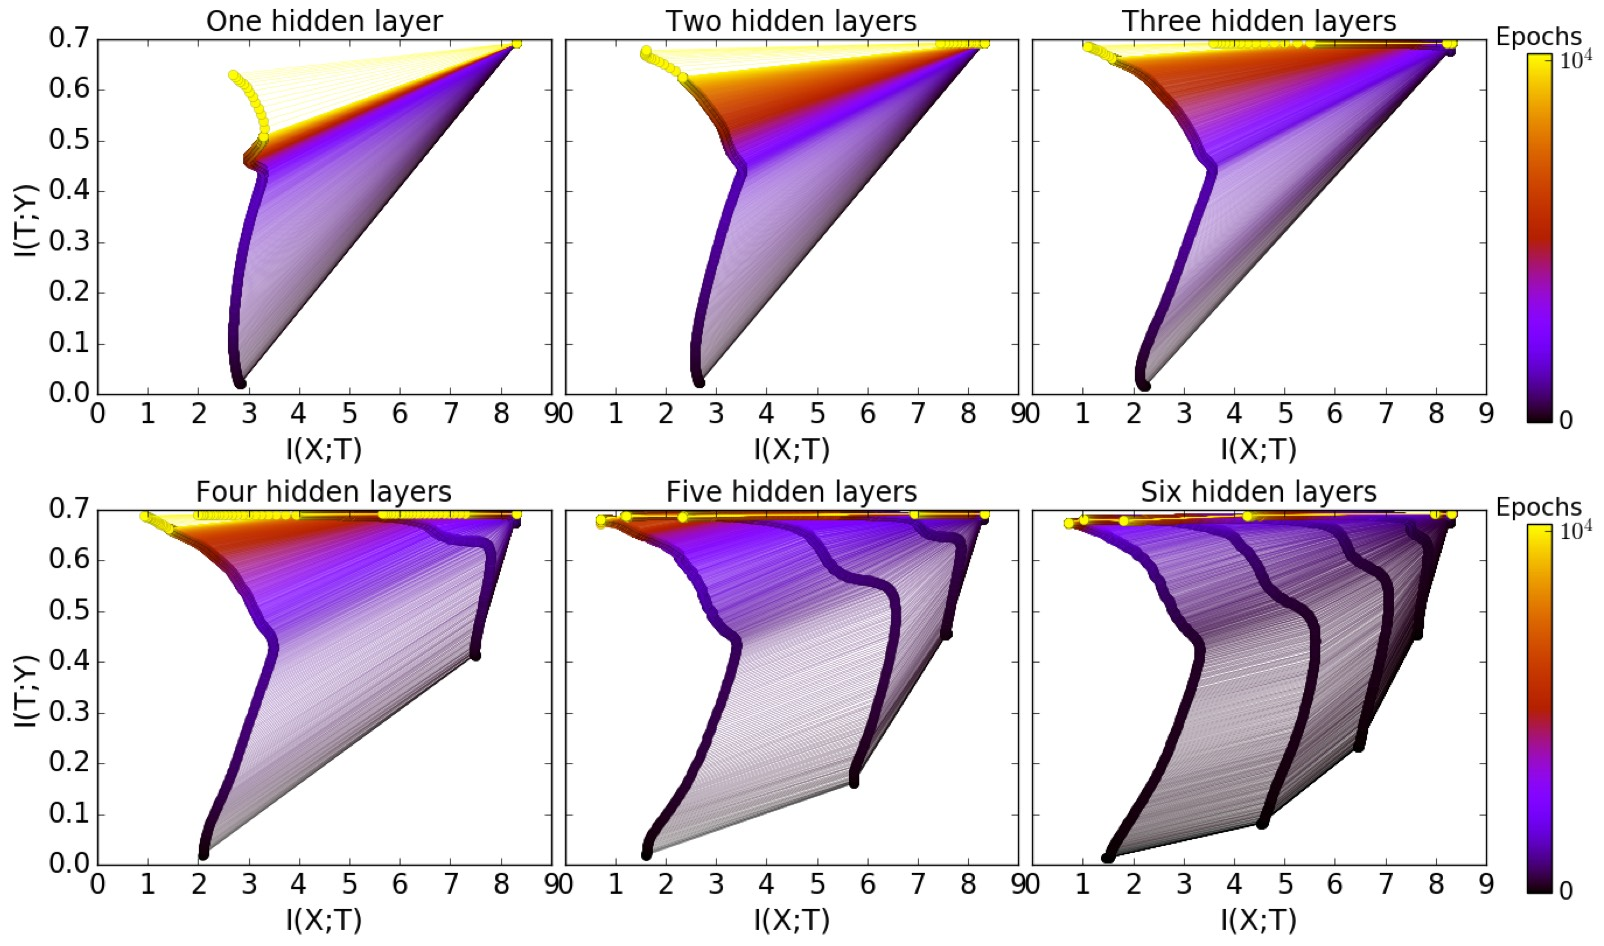
\includegraphics[width=10cm]{info_plane_layers.jpg}
    \end{figure}
    \vspace{-0.4cm}
    The information dynamics of the layers, for different architectures
    \begin{itemize}
        \item Adding layers reduce the training epochs
        \item The compression is faster for deeper layers
    \end{itemize}
\end{frame}

\begin{frame}
    \frametitle{Review of IB}
    \begin{itemize}
        \item DNN learns a bottleneck representation that optimizes the trade-off between compression and prediction
        \item Training DNN undergoes two distinct phases consisting of a fitting phase and a compresssion phase
        \item The compression phase contributes to the generalization performance of DNN
        \item The compression phase occurs due to the diffusion behaviour of SGD
    \end{itemize}
    \vspace{1cm}
    \centering
    \pause \textbf{None of them hold true in the general case!} (\cite{IB-challenge})

\end{frame}

\section{Challenges}

\begin{frame}
    \frametitle{Challenge on the Compression Phase}
    \begin{columns}
        \begin{column}{0.6\textwidth}
            \begin{tikzpicture}[remember picture, overlay]
            % The <2-> makes this node appear only on slide 2
            \node at (current page.south west) [anchor=south west, xshift=-0.05cm, yshift=1cm] {
                \includegraphics[width=8cm]{RELU_results.jpg}
            };
    \end{tikzpicture}
        \end{column}
        \begin{column}{0.4\textwidth}
            \begin{itemize}
                \item (A)(B): binary task
                \item (C)(D): MNIST dataset
                \item (A)(C): DNN with tanh
                \item (B)(D): DNN with ReLU
                \item No compression is observed except the final classification layer using sigmoid neurons
                \item \textbf{Compression arises from the saturation in non-linear activation}
            \end{itemize}
        \end{column}
    \end{columns}
\end{frame}

\begin{frame}
    \frametitle{Challenge on Generalization}
    \begin{columns}
        \begin{column}{0.5\textwidth}
            \begin{tikzpicture}[remember picture, overlay]
            % The <2-> makes this node appear only on slide 2
            \node at (current page.south west) [anchor=south west, xshift=0.25cm, yshift=0.2cm] {
                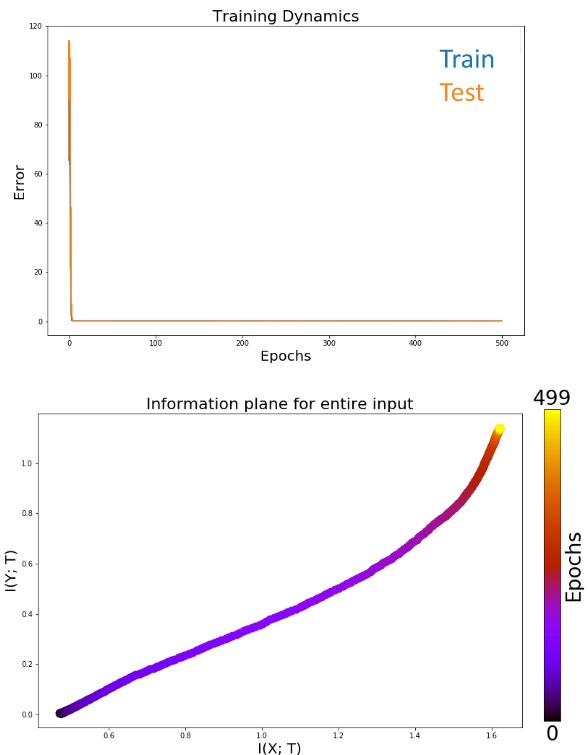
\includegraphics[width=6cm]{no_compression_generalization.jpg}
            };
    \end{tikzpicture}
        \end{column}
        \begin{column}{0.5\textwidth}
            \begin{itemize}
                \item Generalization and information plane in a deep linear network
                \item No compression is observed
                \item The network generalizes well
            \end{itemize}
        \end{column}
    \end{columns}
\end{frame}

\begin{frame}
    \frametitle{Challenge on Diffusion Behaviour}
    \begin{figure}
        \centering
        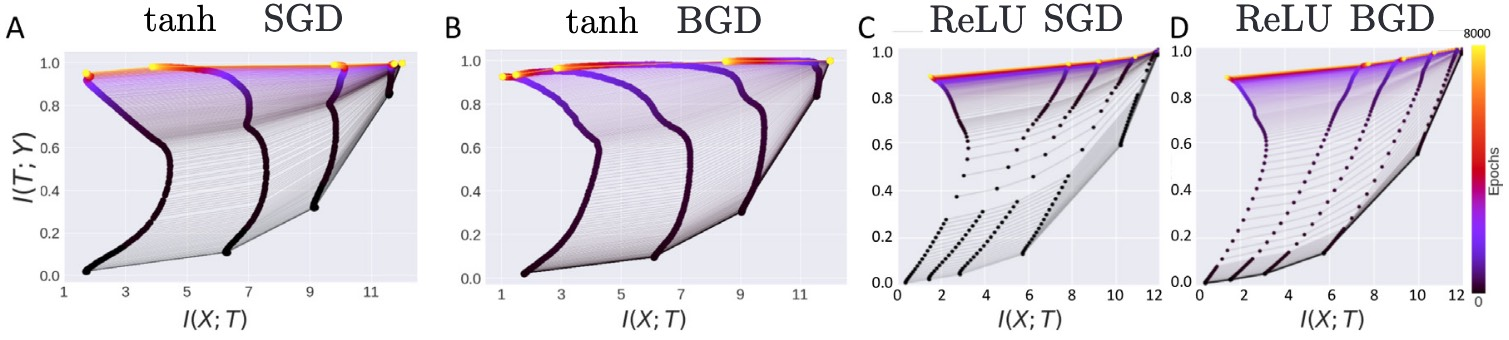
\includegraphics[width=12cm]{BGD.jpg}
    \end{figure}
    \begin{itemize}
        \item SGD: stochastic gradient descent; BGD: full batch gradient descent (no randomness)
        \item The randomness in the training does not contribute to compression of information
    \end{itemize}
    

\end{frame}

%---------------------------------------------------------

% Reference frames
\begin{frame}[allowframebreaks]
    \frametitle{Reference}
    \tiny
    \printbibliography
\end{frame}

%---------------------------------------------------------

\end{document}